\section{Экономическое обоснование проекта}

Проведём расчёт стоимости работ, связанных с разработкой
продукта ConfigtCastle и его дальнейшей эксплуатации.

\tocless\subsection{Экономическая концепция стартапа}

На рисунке \ref{ec:canvas} отображена общая экономическая составляющая стартапа.
Показаны способы привлечения клентов, статьи расходов и так далее.

\begin{figure}[H]
    \center{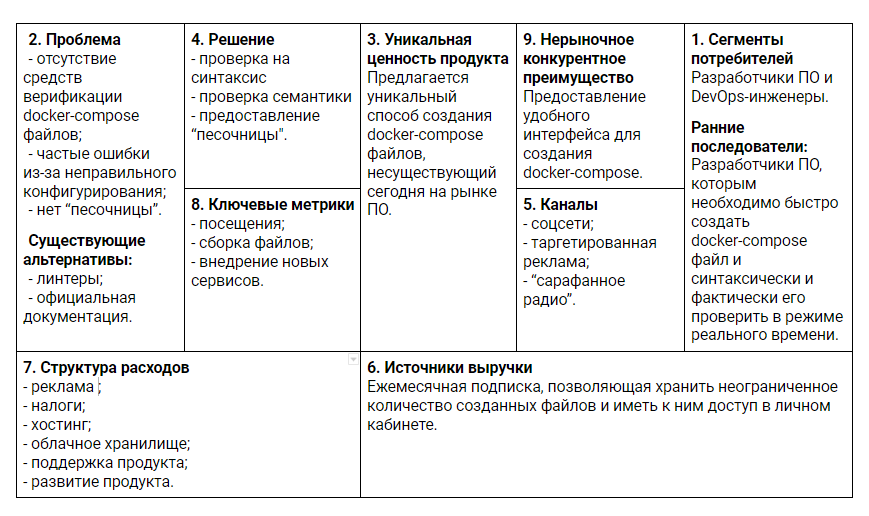
\includegraphics[scale=0.7]{canvas.png}}
    \caption{Экономическое описание стартапа}
    \label{ec:canvas}
\end{figure}

\tocless\subsection{Расчёт прямых расходов}

Прямые расходы включают в себя:
\begin{itemize}
    \item Расходы на оплату труда с учётом трудозатрат;
    \item Страховые взносы во внебюджетные фонды
\end{itemize}

\subsubsection{Расчёт расходов на оплату труда}

Разработкой проекта будут заниматься backend-разработчик и
frontend-разработчик.

Их заработная плата составляет по 30 000 руб. в месяц.

\begin{equation}
   \text{ФОТ}_\text{год} = \text{ЗП} * 12 \text{мес},
\end{equation}

\begin{eqexpl}[25mm]
    \item{ФОТ} Фонд оплаты труда, руб.;
    \item{ЗП} Заработная плата, руб.;
\end{eqexpl}

\begin{equation*}
    \text{ФОТ}_\text{год} = 30 000 * 12 \text{мес.} = 30 000 \text{руб.}
\end{equation*}

Теперь определм стоимость трудозатрат в час по формуле:

\begin{equation}
    \text{Ct}_\text{час} = \text{ФОТ} / N_\text{рв},
\end{equation}

\begin{eqexpl}[25mm]
    \item{$Ct_\text{час}$} Стоимость трудозатрат за 1 час, руб
    \item{$N_\text{рв},$} Норма рабочего времени при 40-ка часовой рабочей
неделе.
\end{eqexpl}

\begin{equation*}
    \text{Ct}_\text{час} = 360 000 / 1979 = 181,91 \text{руб}.
\end{equation*}

Теперь рассчитаем сумму расходов на оплату труда и каждый пункт
разработки занесём в таблицу \ref{ec:table1}

\tabcolsep=0.1cm
\begin{longtable}[c]{|l|c|c|r|}
    \caption{Расчет расходов на оплату труда с учетом трудозатрат}
    \label{ec:table1}\\
    \hline
    \multicolumn{1}{|c|}{{\begin{tabular}[c]{@{}c@{}}Наименование\\ работ/услуг\end{tabular}}} &
      {\begin{tabular}[c]{@{}c@{}}Трудозатраты, \\ час\end{tabular}} &
      {\begin{tabular}[c]{@{}c@{}}Стоимость \\ трудозатрат в час, \\ руб\end{tabular}} &
      {\begin{tabular}[c]{@{}c@{}}Общая стоимость\\ работ, \\ руб\end{tabular}} \\ \hline
    \endfirsthead
    %
    \multicolumn{4}{l}%
    {{Продолжение таблицы \thetable}} \\ \hline
    \endhead
    %
    \begin{tabular}[c]{@{}l@{}}Разработка\\ требований\end{tabular}                              & 72            & 181,91          & 13097,52           \\ \hline
    \begin{tabular}[c]{@{}l@{}}Создание прототипов\\ пользовательского\\ интерфейса\end{tabular} & 16            & 181,91          & 2910,56            \\ \hline
    \begin{tabular}[c]{@{}l@{}}Написание прототипа\\ сервера\end{tabular}                        & 36            & 181,91          & 6548,76            \\ \hline
    Создание дизайна                                                                             & 32            & 181,91          & 5821,12            \\
    \pagebreak
    \begin{tabular}[c]{@{}l@{}}Разработка общей\\ архитектуры проекта\end{tabular}               & 56            & 181,91          & 10186,91           \\ \hline
    Выбор технологий                                                                             & 24            & 181,91          & 4365,84            \\ \hline
    \begin{tabular}[c]{@{}l@{}}Написание кода\\ клиентской части\end{tabular}                    & 496           & 181,91          & 90227,36           \\ \hline
    \begin{tabular}[c]{@{}l@{}}Написание кода\\ серверной части\end{tabular}                     & 456           & 181,91          & 82950,96           \\ \hline
    \begin{tabular}[c]{@{}l@{}}Тестирование клиентской\\ части\end{tabular}                      & 40            & 181,91          & 7276,41            \\ \hline
    \begin{tabular}[c]{@{}l@{}}Тестирование сервеной\\ части\end{tabular}                        & 24            & 181,91          & 4365,84            \\ \hline
    Написание документации                                                                       & 8             & 181,91          & 1455,28            \\ \hline
    \begin{tabular}[c]{@{}l@{}}Изучение документаций к\\ выбранным технологиям\end{tabular}      & 24            & 181,91          & 4365,84            \\ \hline
    Развёртывание на сервере                                                                     & 24            & 181,91          & 4365,84            \\ \hline
    {Итого}                                                                                      & 1308          & 181.91          & 237938,28          \\ \hline
\end{longtable}

\subsubsection{Расчёт страховых взносов во внебюджетные фонды}

Следующим шагом будет определение страховых взносов во внебюджетные фонды, которые состоят
из следующих тарифов:

\begin{itemize}
    \item на обязательное пенсионное страхование ~--- 22,0\%;
    \item на обязательное социальное страхование на случай временной нетрудоспособности и в связи с материнством ~--- 2,9\%;
    \item на обязательное медицинское страхование ~--- 5,1\%;
    \item на обязательное социальное страхование от несчастных случаев на производстве и профессиональных заболеваний ~--- 0.2\%.
\end{itemize}

Для расчёта общих страховых взносов используется следующая формула:

\begin{equation}
    \text{C}_\text{страх-вз} = \text{ФОТ}_\text{год} * 30,2\% / 100\%,
\end{equation}

\begin{eqexpl}[25mm]
    \item{$\text{ФОТ}_\text{год}$} Фонд оплаты труда, руб.
\end{eqexpl}

\begin{equation*}
    \text{C}_\text{страх-вз} = 237938,28 * 30,2\% / 100\% = 71857,36 руб.
\end{equation*}

\tocless\subsection{Определение накладных расходов на разработку программного продукта}

Накладные расходы включают в себя следующие пункты:

\begin{itemize}
    \item Услуги связи(интернет, телефон);
    \item Коммунальные расходы;
    \item Расходы на рекламу;
    \item Прочие
\end{itemize}

Для расчёта накладных расходов рассчитаем временные сроки выполнения проекта по следующей
формуле:

\begin{equation}
    \text{СП} = t_\text{Общ} / 8,
\end{equation}

\begin{eqexpl}[25mm]
    \item{СП} Временные сроки выполнения, дн.;
    \item{$t_\text{общ}$} Общая сумма трудозатрат, час;
    \item{8} Стандартный рабочий день, час.
\end{eqexpl}

\begin{equation*}
    \text{СП} = 1308 / 8 = 163,5 дн.
\end{equation*}

\subsubsection{Расчёт расходов на услугуи связи}

Расчёт расходов на связь можно посчитать по следующей формуле:

\begin{equation}
    \text{P}_\text{y.c.} = (\text{P}_\text{интернет} + \text{P}_\text{тел.связь}) / \text{Кол-во дней(мес)} * \text{СП},
\end{equation}

\begin{eqexpl}[57mm]
    \item{$P_\text{интернет} + P_\text{тел.связь}$} Расходы на интернет, мобильную связь и т.д.;
    \item{Кол-во дней(мес)} Среднее количество рабочий дней в месяце, дн.
\end{eqexpl}

\begin{equation*}
    \text{P}_\text{y.c.} = (450 + 300 + 400 + 300) / 21 * 163,5 = 11289,29 руб.
\end{equation*}

\subsubsection{Расчёт расходов на коммунальные услуги}

Расчёт коммунальных услуг произведём по формуле:

\begin{equation}
    P_\text{коммунальные} = n_\text{к.у} * S,
\end{equation}

\begin{eqexpl}[25mm]
    \item{$P_\text{коммунальные}$} Расходны на коммунальные услуги;
    \item{$n_\text{к.у}$} Средняя ставка на ком. услуги за 1 кв. метр;
    \item{$S$} Площадь помещения в кв. м.
\end{eqexpl}

\begin{equation*}
    P_\text{коммунальные} = 120 * 30 = 3600 \text{руб}.
\end{equation*}

\subsubsection{Расчёт расходов на рекламу}

Произведём расчёт расходов на рекламу по следующей формуле:

\begin{equation}
    P_\text{реклама} = POT * n_\text{реклама} / 100\%,
\end{equation}

\begin{eqexpl}[25mm]
    \item{$P_\text{реклама}$} Сумма расходов на рекламу, руб.;
    \item{$POT$} Расходы на оплату труда, руб.;
    \item{$n_\text{реклама}$} Норматив расходов на рекламу, руб.
\end{eqexpl}

\begin{equation*}
    P_\text{реклама} = 237938,28 * 10\% / 100\% = 23793,83 \text{руб}.
\end{equation*}

\subsubsection{Расчёт прочих расходов}

Рассчитаем расходы на оплату труда, которые являются процентом от расходов
на оплату труда как и расходы на рекламу, по формуле:

\begin{equation}
    P_\text{прочие} = POT * n_\text{прочие} / 100\%,
\end{equation}

\begin{eqexpl}[25mm]
    \item{$P_\text{прочие}$} Сумма прочих расходов, руб.;
    \item{$n_\text{прочие}$} Норматив прочих расходов, \%
\end{eqexpl}

\begin{equation*}
    P_\text{прочие} =  237938,28 * 10\% / 100\% = 23793,83 \text{руб}.
\end{equation*}

\subsubsection{Расчёт общей суммы накладных расходов}

Теперь можно определить общую сумма накладных расходов по следующей формуле:

\begin{equation}
    P_\text{Накладные} = P_y.c. + P_\text{коммунальные} + P_\text{реклама} + P_\text{прочие}.
\end{equation}

\begin{eqexpl}[25mm]
    \item{$P_\text{Накладные}$} Сумма накладных расходов, руб.
\end{eqexpl}

\begin{equation*}
    P_\text{Накладные} = 11289,29 + 3600 + 23793,83 * 2 = 62476,95 \text{руб.}
\end{equation*}

\tocless\subsection{Расчёт себестоимости работ по разработке программного продукта}

Себестоимость работ по проекту включает в себя:

\begin{itemize}
    \item Расходы на оплату труда;
    \item Страховые взносы;
    \item Накладые расходы.
\end{itemize}

Расчёт себестоимости работ по проекту, иными словами цену непосредственного создания
программного продукта, привидена в таблице \ref{ec:table2}.

\tabcolsep=0.5cm
\begin{longtable}[c]{|l|c|}
    \caption{Себестоимость работ по созданию программного продукта}
    \label{ec:table2}\\
    \hline
    \multicolumn{1}{|c|}{{Статьи расходов}} & {\begin{tabular}[c]{@{}c@{}}Сумма, руб.\end{tabular}} \\ \hline
    \endfirsthead
    %
    \multicolumn{2}{c}%
    {{Продолжение таблицы \thetable}} \\
    \endhead
    %
    Расход на оплату труда & 237938,28          \\ \hline
    Страховые взносы       & 71857,36           \\ \hline
    Накладные расходы      & 62476,95           \\ \hline
    {Итого}         & {372272,59} \\ \hline
\end{longtable}

\tocless\subsection{Расчёт сумму выручки от реализации программного продукта}

Цена создания и реализации программного продукта ~--- она же выручка от
реализации проекта определяется по следующей формуле:

\begin{equation}
    B_\text{реал} = C_p + \text{П},
\end{equation}

\begin{eqexpl}[25mm]
    \item{$C_p$} Себестоимость работ, руб.;
    \item{П} Планируемый размер прибыли, руб.
\end{eqexpl}

Планируемый размер прибыли определяется по следующей формуле:

\begin{equation}
    \text{П} = \frac{C_p * H_r}{100\%},
\end{equation}

\begin{eqexpl}[25mm]
    \item{$H_R$} Уровень рентабельности проекта, \%.
\end{eqexpl}

Возьмём за уровень рентабельности 10\%, так как проект не прибыльный по своей сути.

\begin{equation*}
    \text{П} = \frac{372272.59 * 10\%}{100\%} = 37227.259 \text{руб}.
\end{equation*}

Следовательно:

\begin{equation*}
    B_\text{реал} = 372272,59 + 37137.259 = 409499,849 \text{руб.},
\end{equation*}

Основные же показатели, учитываемые при расчётё цены программного продукта привидены в таблице
\ref{ec:table3}

\begin{longtable}[c]{|l|r|}
    \caption{Расчет цены программного продукта}
    \label{ec:table3}\\
    \hline
    \multicolumn{1}{|c|}{{Наименование показателя}} & {Сумма, руб} \\ \hline
    \endfirsthead
    %
    \multicolumn{2}{c}%
    {{Продолжение таблицы \thetable}} \\
    \endhead
    %
    Затраты на создание программного продукта              & 371372,59           \\ \hline
    Прибыль                                                & 37227,259           \\ \hline
    Выручка от реализации проекта                          & 409499,84           \\ \hline
\end{longtable}

\tocless\subsection{Расчёт суммы единого налога при применении упрощённой системы налогообложения}

Произведём расчёт суммы единого налога по формуле:

\begin{equation}
    \text{УСН}_\text{нач} = \frac{\text{Д} * C_\text{усн}}{100\%},
\end{equation}

\begin{eqexpl}[25mm]
    \item{$\text{УСН}_\text{нач}$} Сумма единого налогового начисления, руб.;
    \item{Д} Доход, руб.;
    \item{$C_\text{усн}$} Ставка налога, \%.
\end{eqexpl}

\begin{equation*}
    \text{УСН}_\text{нач} = \frac{37227,259 * 6\%}{100\%} = 2233,64 \text{руб}.
\end{equation*}

Налогоплательщики, выбравшие в качестве объекта налогообложения
доходы, уменьшают сумму налога, исчисленную за налоговый период, на
сумму страховых взносов, но не более, чем на 50\%.

Определим сумму минимального налога по формуле:

\begin{equation}
    \text{УСН}_\text{min} = \frac{\text{УСН}_\text{нач} * 50\%}{100\%},
\end{equation}

\begin{eqexpl}[25mm]
    \item{$\text{УСН}_\text{min}$} Минимальная сумма налога, руб.
\end{eqexpl}

\begin{equation*}
    \text{УСН}_\text{min} = \frac{2233,64 * 50\%}{100\%} = 1116,82 руб.
\end{equation*}

Произведем расчет суммы единого налога, подлежащей перечислению
в бюджет по формуле:

\begin{equation}
    \text{УСН}_\text{бюджет} = \text{УСН}_\text{нач} - \text{УСН}_min
\end{equation}

\begin{equation}
    \text{УСН}_\text{бюджет} = 2233,64 - 1116,82 = 1116,82 руб.
\end{equation}

\tocless\subsection{Расчёт чистой прибыли организации}

Рассчитаем сумму чистой прибыли, остающаяся в распоряжении организации,
после уплаты единого налога по формуле:

\begin{equation}
    \text{П}_\text{чистая} = П - \text{УСН}_\text{бюджет},
\end{equation}

\begin{eqexpl}[25mm]
    \item{$\text{П}_\text{чистая}$} Планируемая сумма прибыли от реализации проекта, руб.
\end{eqexpl}

\begin{equation*}
    \text{П}_\text{чистая} = 37227,259 - 1116,82 = 36110,44 руб
\end{equation*}

Расчет чистой прибыли организации от разработки программного
продукта сведём в таблицу \ref{ec:table4}

\begin{longtable}[c]{|l|r|}
    \caption{Расчёт чистой прибыли организации от разработки
    программного продукта.}
    \label{ec:table4}\\
    \hline
    \multicolumn{1}{|c|}{{Наименование статей}} & {Сумма, руб} \\ \hline
    \endfirsthead
    %
    \multicolumn{2}{c}%
    {{Продолжение таблицы \thetable}} \\
    \endhead
    %
    Себестоимость работ по проекту                     & 372272,59          \\ \hline
    Планируемая сумма прибыли                          & 37227,259           \\ \hline
    Выручка от реализации проекта                      & 409499,849          \\ \hline
    Сумма единого налога, подлежащая уплате в бюджет   & 1116,82            \\ \hline
    \begin{tabular}[c]{@{}l@{}}Прибыль, остающаяся в распоряжении организации,\\ после уплаты единого налога при применении УСН\end{tabular} & 36110.44 \\ \hline
\end{longtable}

\tocless\subsection{Расчёт стоимости владения программным продуктом}

Стоимость владени программным продуктом включает в себя
эксплуатационные расходы (Эр) на обслуживание разработанного
программного продукта (таблица \ref{ec:table5}), измеряются в часах, затраченных на
указанные ниже виды работ.

Ежемесячные затраты на функционирование (Зф) программного
продукта (таблица \ref{ec:table6}) так же входят в стоимость владения программным
продуктом.

\tabcolsep=0.1cm
\begin{longtable}[c]{|l|c|c|r|}
    \caption{Расчет эксплуатационных расходов.
    }
    \label{ec:table5}\\
    \hline
    \multicolumn{1}{|c|}{{Наименование статей}} &
      \begin{tabular}[c]{@{}c@{}}Количество\\ часов,\\ час/мес\end{tabular} &
      \begin{tabular}[c]{@{}c@{}}Стоимость\\ трудозатрат в\\ час, \\ руб.\end{tabular} &
      \begin{tabular}[c]{@{}c@{}}Сумма,\\ руб. в месяц\end{tabular} \\ \hline
    \endfirsthead
    %
    \multicolumn{4}{c}%
    {{Продолжение таблицы \thetable}} \\
    \endhead
    %
    Создание новых сервисов                                                                                         & 24          & 181.91          & 4365,84           \\ \hline
    Оптимизация производительсности                                                                                 & 10          & 181.91          & 1819,1            \\ \hline
    \begin{tabular}[c]{@{}l@{}}Установка и тестирование\\ программных обновлений\\ разработотанного ПО\end{tabular} & 5           & 181.91          & 909,55            \\ \hline
    Модерация ресурсов                                                                                              & 30          & 181.91          & 5457,3            \\ \hline
    Итого                                                                                                  & 69 & 181.91 & 12551.79 \\ \hline
\end{longtable}

\begin{longtable}[c]{|l|r|}
    \caption{Расчет затрат на функционирование.
    }
    \label{ec:table6}\\
    \hline
    \multicolumn{1}{|c|}{{Виды затрат}}                                              & \begin{tabular}[c]{@{}c@{}}Сумма,\\ руб./месяц\end{tabular} \\ \hline
    \endfirsthead
    %
    \multicolumn{2}{c}%
    {{Продолжение таблицы \thetable}} \\
    \endhead
    %
    Стоимость домена   & 590           \\ \hline
    Стоимость хостинга & 825           \\ \hline
    \begin{tabular}[c]{@{}l@{}}Стоимость облачного\\ сервиса базы данных(mLab)\end{tabular} & 545                                                                  \\ \hline
    {Итого}     & {1960} \\ \hline
\end{longtable}

Итого, стоимость владения (Св) рассчитывается как сумма
эксплуатационных расходов и затрат на функционирование по формуле:

\begin{equation}
    C_\text{в} = \text{Э}_\text{р} + \text{З}_\text{ф}.
\end{equation}

\begin{equation*}
    C_\text{в} = 12551,79 + 1960 = 14511,79 руб.
\end{equation*}

Вывод: стоимость владения разработанным продуктом, составляет 14511,79 руб. в месяц.

\tocless\subsection{Смета затрат на проект}

Смета затрат на проект включает в себя себестоимость проекта,
заложенную сумму прибыли разработчика, сумму налоговых платежей.
Отдельной строкой необходимо указать стоимость владения программным
продуктом. Расчёт сметы представлен в таблице \ref{ec:table7}

\begin{longtable}[c]{|l|l|r|}
    \caption{Смета затрат на проект.}
    \label{ec:table7}\\
    \hline
    \multicolumn{1}{|c|}{{\begin{tabular}[c]{@{}c@{}}№\\ п/п\end{tabular}}} &
      \multicolumn{1}{c|}{{Статьи смета затрат на проект}} &
      {\begin{tabular}[c]{@{}l@{}}Сумма,\\ руб.\end{tabular}} \\ \hline
    \endfirsthead
    %
    \multicolumn{3}{c}%
    {Продолжение таблицы \thetable} \\
    \endhead
    %
    1 &
      \begin{tabular}[c]{@{}l@{}}Затратны на создание программного\\ продукта(себестоимость работ)\end{tabular} &
      372272,59 \\ \hline
                         & Расходы на оплату труда               & 237938,28  \\ \hline
                         & Страховые взносы                      & 71857,36   \\ \hline
                         & Накладные расходы                     & 62476,95   \\ \hline
    2                    & Чистая прибыль                        & 36110,44  \\ \hline
    3                    & Налог по УСН с выручки                & 1116,12    \\ \hline
    \multicolumn{2}{|l|}{Итого общая стоимость работ по проекту} & 409509,86 \\ \hline
    4                    & Стомость владения ПП, месяц           & 14511,79   \\ \hline
\end{longtable}
